\section{Resultados e discussão}\label{sec:results}

\subsection{Convergência e dispersão entre sementes}\label{sec:res_ruido}

As 1800 execuções do NSGA-II, correspondentes aos 360 casos da campanha com cinco sementes cada, terminaram com fronteiras viáveis. A dispersão do volume mínimo entre as sementes de um mesmo caso, $100\,(V_{\max}/V_{\min}-1)$, tem mediana de 1,48\%, percentil 90 de 4,07\% e máximo de 9,88\%, este na guaiçara com vão de 10~m. Uma execução isolada carrega, portanto, um erro de otimização da mesma ordem das diferenças de volume que o estudo procura medir, o que justifica a adoção do menor volume entre cinco sementes (Seção~\ref{sec:sementes}). A semente que produziu esse menor volume varia de caso para caso, sem que nenhuma predomine: as sementes 1 a 5 foram as melhores em 56, 76, 59, 95 e 74 casos, respectivamente.

A dispersão entre sementes revela também um aspecto da própria solução ótima. Em 309 dos 360 casos, a verificação de maior utilização não é a mesma em todas as sementes. Na solução de menor volume, a flexão do tabuleiro, a flexão da longarina e, nos vãos maiores, a flecha ficam simultaneamente a menos de 1 a 2\% do limite, e diferenças pequenas entre execuções alternam o rótulo da verificação governante sem mudar o volume de forma relevante. Esse rótulo não é, assim, um descritor estável do projeto, e o regime de cada par é definido pela utilização da flecha, como descrito na Seção~\ref{sec:escala}.

Nenhuma solução encostou em limite de domínio do intervalo de busca. Dezessete casos têm alguma variável na borda do intervalo, todos em limites construtivos: em doze casos de espécie com vão de 3~m, a prancha do tabuleiro fica na espessura mínima de 5~cm, e em cinco casos o espaçamento entre pranchas fica no mínimo ou no máximo admissível. Nos vãos de 3 a 6~m, a base de classes reproduz a campanha de semente única da plataforma com diferenças entre $-5{,}4\%$ e $+0{,}3\%$ e mediana de $-1{,}3\%$. O sinal predominantemente negativo indica que a busca com cinco sementes alcança projetos mais leves que a execução única, o que confirma, em outra população de casos, a ordem de grandeza do erro de otimização medido acima.

\subsection{Base de classes: volume e regime governante}\label{sec:res_classes}

A Figura~\ref{fig:res_base_classes}a apresenta o volume do projeto pela classe em função do vão. O volume cresce com o vão segundo uma lei de potência de expoente entre 1,62 e 1,69, próxima da obtida anteriormente na faixa de 3 a 6~m, e o projeto em D20 consome de 1,64 a 1,80 vez o volume do projeto em D60 no mesmo vão.

\begin{figure}[!ht]
\centering
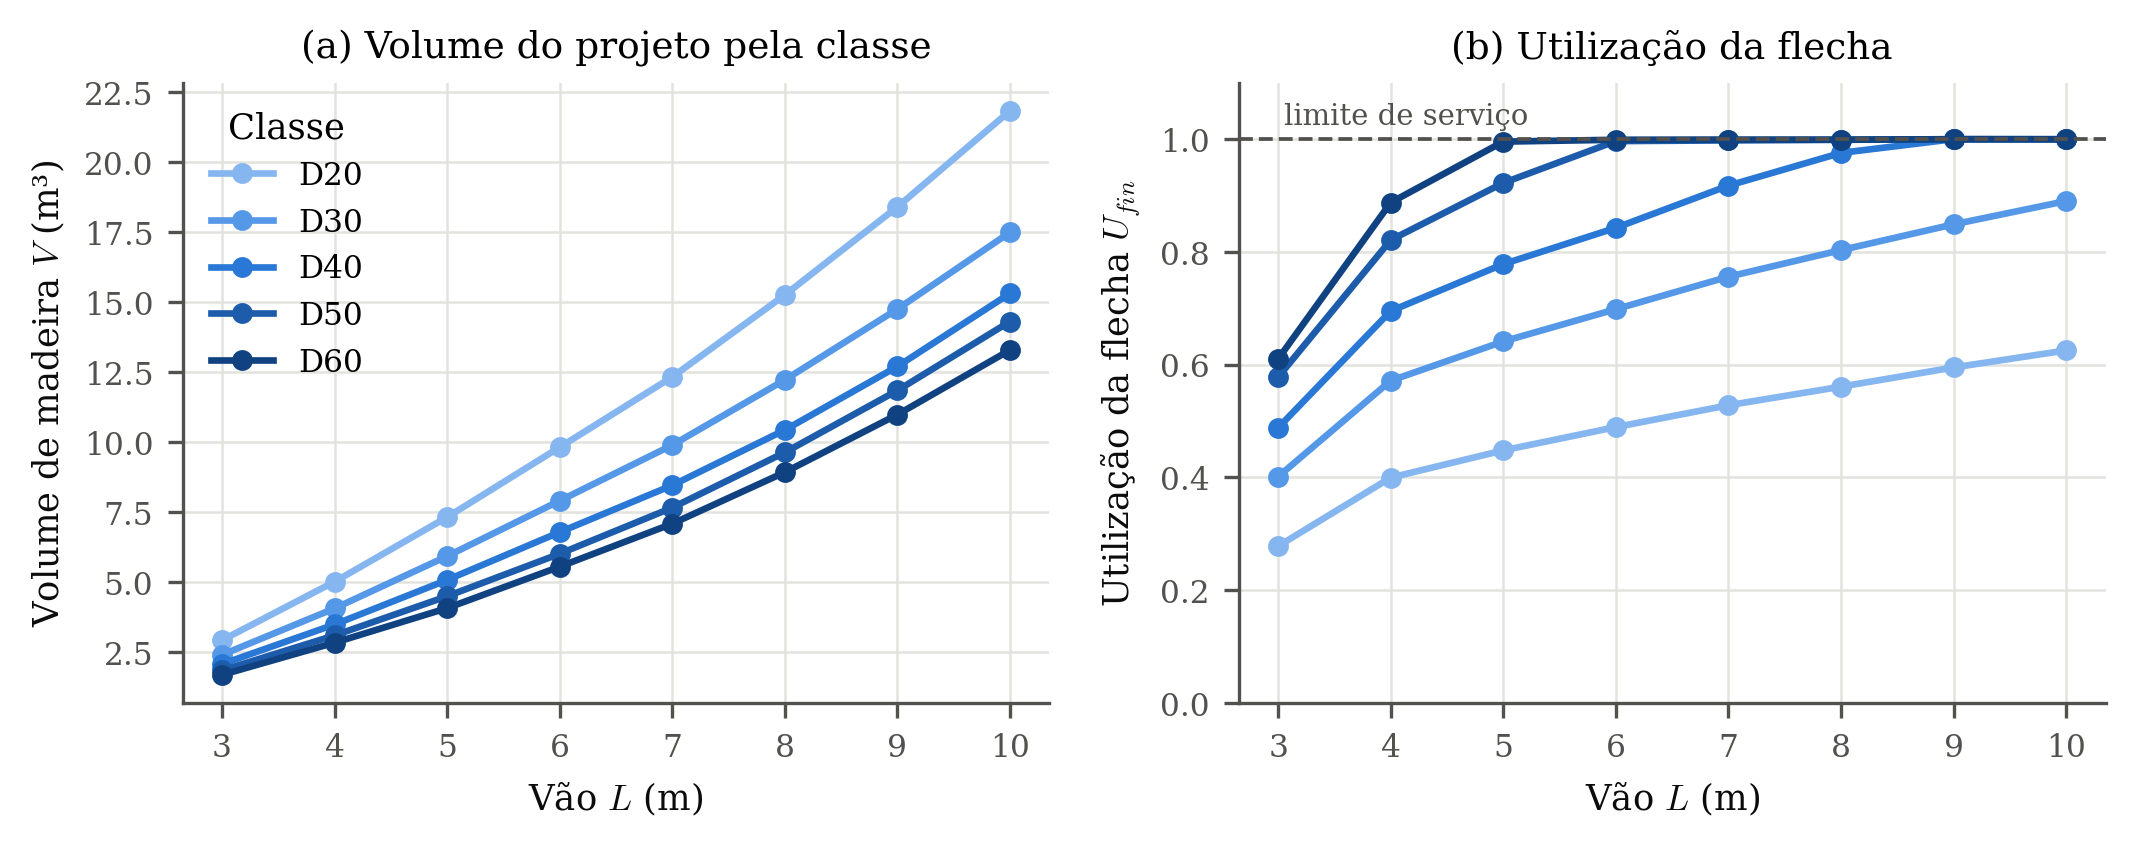
\includegraphics[width=\textwidth]{figuras/res_base_classes.png}
\caption{Base de classes: (a) volume de madeira da solução de menor volume e (b) utilização da flecha final $U_{fin}$ dessa solução, em função do vão, por classe de resistência.}
\label{fig:res_base_classes}
\end{figure}

A Figura~\ref{fig:res_base_classes}b mostra que o regime governante depende da classe tanto quanto do vão. Nas classes D20 e D30, a flecha não chega ao limite em nenhum vão estudado, com utilizações de 0,63 e 0,89 em 10~m, e o projeto é governado por resistência em toda a faixa. Nas classes superiores, a flecha torna-se ativa cada vez mais cedo: a partir de 9~m na D40, de 6~m na D50 e de 5~m na D60. A ordem decorre da própria definição das classes. A resistência de referência triplica de D20 para D60, enquanto o módulo de elasticidade não chega a dobrar, de modo que a razão $E_{c0,m}/f_{c0,k}$ cai de 500 na D20 para 325 na D60. Quanto mais alta a classe, menor a seção que a resistência exige e mais cedo a rigidez passa a condicionar o projeto. Como consequência, a comparação entre uma espécie e a sua classe ocorre em regimes diferentes conforme a classe e o vão, o que antecipa que um único coeficiente não descreve o efeito da representação por classe em toda a campanha.

\subsection{Diferença de volume entre o projeto pela espécie e pela classe}\label{sec:res_deltaV}

A Tabela~\ref{tab:res_vao} resume, por vão, a diferença de volume $\Delta V$ entre o projeto pela classe e o projeto pela espécie. Nos 320 pares, $\Delta V$ tem mediana de 4,5\% e varia de $-15{,}0\%$ a $+23{,}1\%$. No vão de 3~m, todos os pares são positivos, entre 0,3\% e 23,1\%: o projeto pela classe consome mais madeira em qualquer espécie. À medida que o vão cresce, a mediana cai de 6,8\% em 3~m para 1,5\% em 10~m, mas a distribuição se alarga para valores negativos, que aparecem a partir de 4~m e chegam a 18 dos 40 pares em 9 e 10~m.

\begin{table}[!ht]
\centering
\caption{Diferença de volume $\Delta V=V_{cls}/V_{esp}-1$ entre o projeto pela classe e o projeto pela espécie, e reavaliação do projeto pela classe com as propriedades da espécie, por vão (40 pares por vão).}
\label{tab:res_vao}
\footnotesize
\setlength{\tabcolsep}{4pt}
\begin{tabular}{rrrrrrrr}
\toprule
 & \multicolumn{3}{c}{$\Delta V$ (\%)} & & \multicolumn{2}{c}{Viola o ELS} & Espécie \\
\cmidrule(lr){2-4}\cmidrule(lr){6-7}
$L$ (m) & Mediana & $Q_1$ a $Q_3$ & Mín.\ a máx. & $\Delta V<0$ & Robusto & Nominal & economiza $>5\%$ \\
\midrule
3 & 6{,}8 & 4{,}3 a 10{,}2 & 0{,}3 a 23{,}1 & 0 & 0 & 0 & 26 \\
4 & 5{,}4 & 3{,}4 a 10{,}1 & $-$6{,}9 a 21{,}1 & 4 & 6 & 1 & 24 \\
5 & 4{,}8 & 0{,}2 a 9{,}4 & $-$9{,}3 a 20{,}9 & 9 & 11 & 3 & 19 \\
6 & 4{,}2 & 0{,}2 a 8{,}9 & $-$11{,}1 a 22{,}0 & 10 & 13 & 4 & 19 \\
7 & 3{,}6 & $-$0{,}7 a 8{,}5 & $-$12{,}5 a 22{,}2 & 12 & 15 & 5 & 15 \\
8 & 2{,}6 & $-$1{,}3 a 8{,}0 & $-$13{,}5 a 22{,}4 & 15 & 18 & 6 & 15 \\
9 & 1{,}6 & $-$2{,}0 a 7{,}9 & $-$14{,}3 a 22{,}5 & 18 & 21 & 7 & 15 \\
10 & 1{,}5 & $-$2{,}7 a 8{,}2 & $-$15{,}0 a 22{,}5 & 18 & 21 & 7 & 15 \\
\midrule
Total & 4{,}5 & $-$0{,}4 a 9{,}4 & $-$15{,}0 a 23{,}1 & 86 & 105 & 33 & 148 \\
\bottomrule
\end{tabular}
\begin{minipage}{0.95\linewidth}\vspace{2pt}\footnotesize
``Robusto'': alguma verificação excede o limite no pior caso da grade de $\pm5\%$ no diâmetro, que é o critério de aceitação da campanha. ``Nominal'': excede com o diâmetro nominal. ``Espécie economiza'': projeto pela classe seguro e $\Delta V>5\%$.
\end{minipage}
\end{table}

Os valores negativos têm uma interpretação precisa, que a reavaliação da Seção~\ref{sec:res_seguranca} torna explícita. Os 86 pares em que o projeto pela classe usa menos madeira que o projeto pela espécie estão todos entre os pares em que o projeto pela classe viola o limite de serviço quando reavaliado com as propriedades da espécie. Nesta campanha, o projeto pela classe só economiza madeira quando é inadequado para a espécie. Nos 215 pares em que ele é admissível, $\Delta V$ é sempre positivo, com mediana de 6,9\% e máximo de 23,1\%.

\subsection{Reavaliação do projeto pela classe e critério de segurança}\label{sec:res_seguranca}

Reavaliado com as propriedades da espécie, o projeto pela classe viola algum estado limite em 105 dos 320 pares no critério de aceitação da campanha, que é o pior caso da grade de $\pm5\%$ no diâmetro, e em 33 pares com o diâmetro nominal (Tabela~\ref{tab:res_vao}). A verificação violada é sempre a flecha da longarina. As verificações de resistência nunca são excedidas, com utilizações máximas de 0,983 na flexão da longarina, 0,986 na flexão do tabuleiro e 0,493 no cisalhamento, o que é consequência direta do enquadramento: como a classe é atribuída pelo piso de $f_{c0,k}$, a resistência da espécie nunca é inferior à da classe. O risco introduzido pela representação por classe está, assim, inteiramente na rigidez.

O número de violações cresce com o vão, de nenhuma em 3~m para 21 em 9 e 10~m, acompanhando a entrada das classes superiores no regime de flecha. Nos vãos de 9 e 10~m, 21 das 23 espécies com módulo inferior ao da classe produzem violação. As duas exceções pertencem à classe D20, cujo projeto mantém folga de flecha em toda a faixa estudada. Entre os pares que violam o limite, a utilização da flecha reavaliada tem mediana de 1,13 e chega a 1,59, isto é, a flecha do projeto construído com a espécie supera em até 59\% o limite de serviço que o projeto pela classe pretendia atender.

A Figura~\ref{fig:res_limiar}b compara essa utilização reavaliada com a previsão da Equação~\eqref{eq:u_ctor}. O ajuste de $U_{fin}^{C\rightarrow R}/U_{fin,cls}$ às razões de rigidez e de densidade resulta em expoente de $1{,}002\pm0{,}004$ para $E_{c0,m}^{\mathrm{NBR}}/E_{c0,m}^{\mathrm{exp}}$ e de $0{,}090\pm0{,}005$ para $\rho_{ap}^{\mathrm{exp}}/\rho_{ap}^{\mathrm{NBR}}$, com $R^2=0{,}999$ e erro quadrático médio de 0,55\%. A flecha do projeto pela classe responde, portanto, à razão de módulos na proporção exata prevista pela Equação~\eqref{eq:razao_delta}, e a troca de densidade tem efeito de segunda ordem.

\begin{figure}[!ht]
\centering
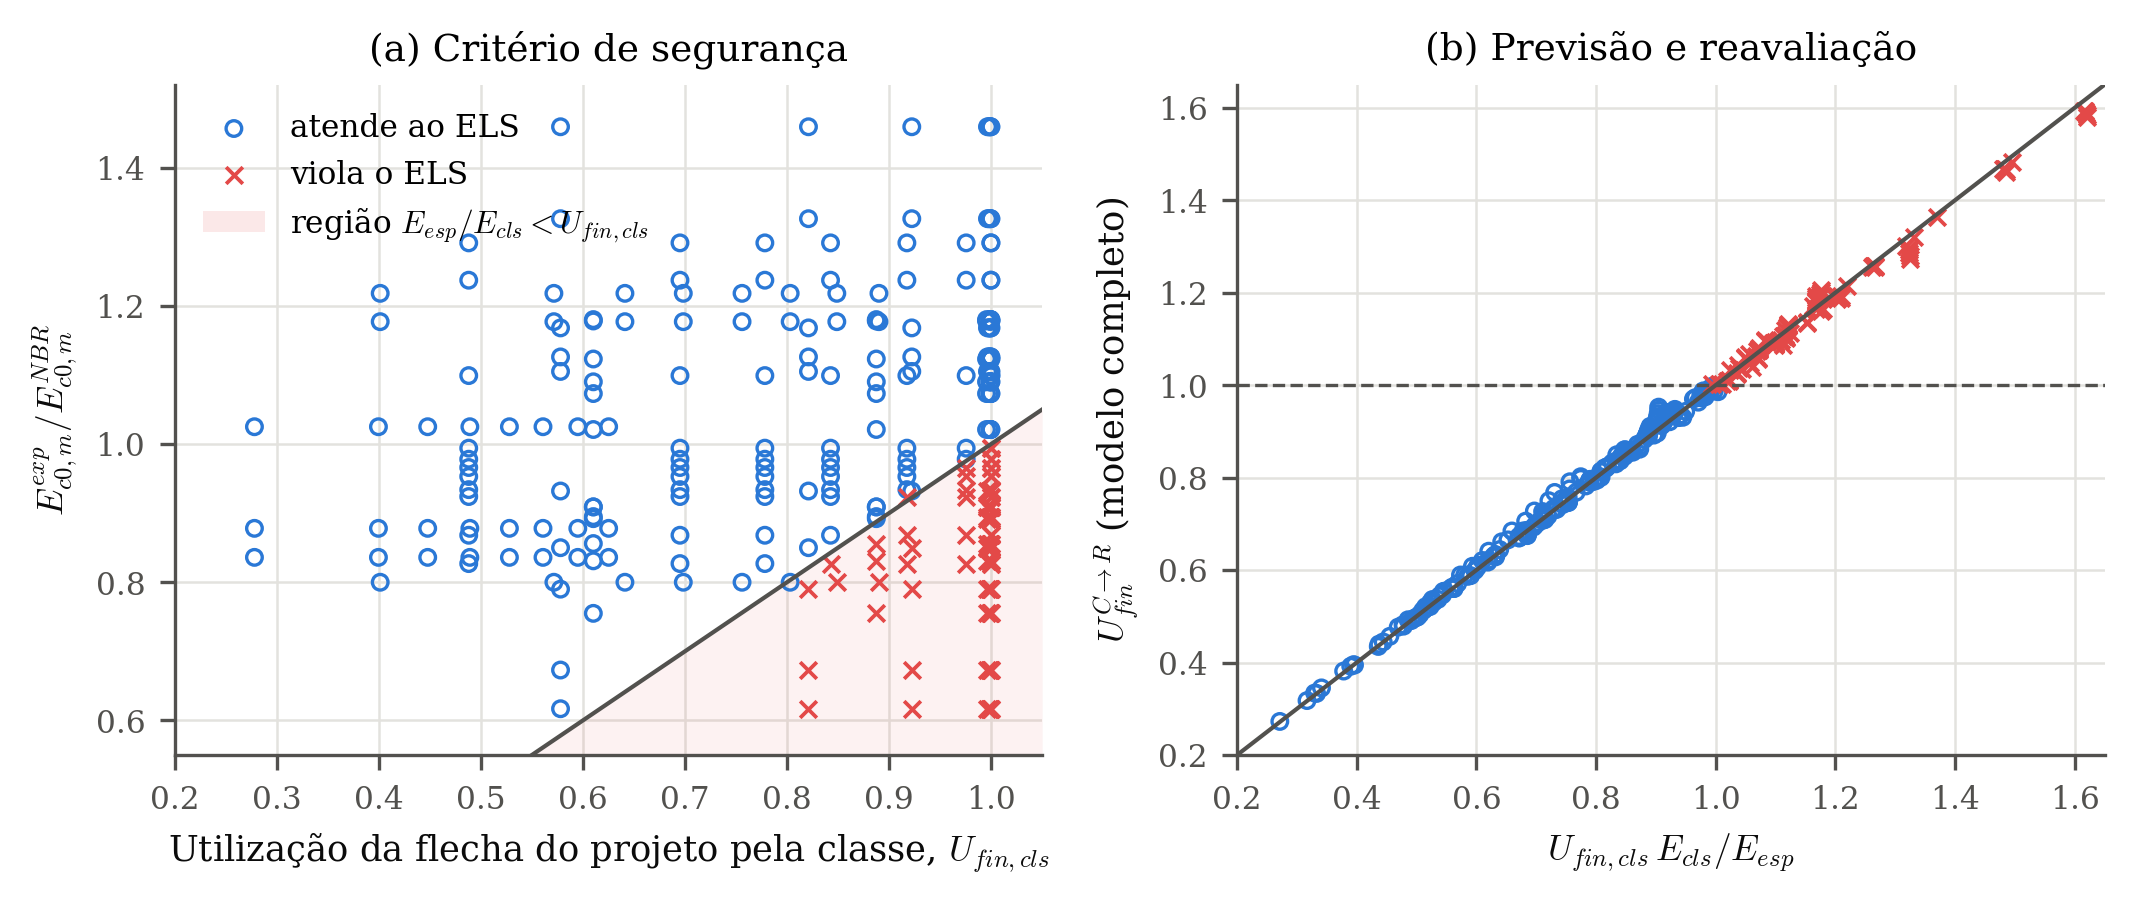
\includegraphics[width=\textwidth]{figuras/res_limiar_seguranca.png}
\caption{Atendimento ao limite de serviço do projeto pela classe reavaliado com as propriedades da espécie: (a) critério da Equação~\eqref{eq:criterio}, com a razão de módulos da espécie contra a utilização da flecha do projeto pela classe; (b) utilização reavaliada pelo modelo completo contra a previsão da Equação~\eqref{eq:u_ctor}. Cada marcador é um par espécie--vão.}
\label{fig:res_limiar}
\end{figure}

O critério da Equação~\eqref{eq:criterio} classifica corretamente 318 dos 320 pares (Figura~\ref{fig:res_limiar}a). Os dois erros ficam na fronteira do critério e são explicados pela densidade, que a Equação~\eqref{eq:criterio} desconsidera. O piolho em 7~m, com densidade 10,4\% acima da classe, excede o limite em 0,2\%, embora o critério o classifique como admissível. O cedro-amargo em 8~m, com densidade 17,8\% abaixo da classe, fica 1,4\% abaixo do limite, embora o critério o classifique como inadmissível. O critério exige apenas a utilização da flecha do projeto pela classe, que o projetista obtém no próprio dimensionamento, e a razão de módulos da espécie. Quando essa razão é desconhecida, o menor valor observado entre as espécies da classe delimita a faixa de vãos em que o projeto pela classe atende a todas as espécies da base: até 10~m na D20, 8~m na D30, 5~m na D40 e apenas 3~m nas classes D50 e D60, em que as espécies menos rígidas têm módulo 38\% e 25\% inferior ao da classe.

\subsection{Leis de escala da diferença de volume}\label{sec:res_escala}

A Tabela~\ref{tab:res_regressao} apresenta os expoentes da Equação~\eqref{eq:regressao} por regime. O ajuste conjunto dos 320 pares explica apenas 66\% da variância de $\ln(V_{cls}/V_{esp})$, com erro quadrático médio de 4,1\%. Separados por regime, os ajustes explicam de 95\% a 98\% da variância, e os expoentes mudam de forma coerente com a mecânica do problema.

\begin{table}[!ht]
\centering
\caption{Expoentes do ajuste $\ln(V_{cls}/V_{esp})=b_f\ln(1+\Delta_f)+b_E\ln(1+\Delta_E)+b_\rho\ln(1+\Delta_\rho)$ por regime, com intervalos de confiança de 95\%.}
\label{tab:res_regressao}
\footnotesize
\begin{tabular}{lrrrrrr}
\toprule
Regime & $n$ & $b_f$ & $b_E$ & $b_\rho$ & $R^2$ & RMSE (\%) \\
\midrule
Resistência & 109 & 0{,}507 $\pm$ 0{,}014 & 0{,}005 $\pm$ 0{,}016 & 0{,}004 $\pm$ 0{,}021 & 0{,}955 & 1{,}24 \\
Flecha & 137 & 0{,}160 $\pm$ 0{,}008 & 0{,}322 $\pm$ 0{,}009 & $-$0{,}037 $\pm$ 0{,}014 & 0{,}984 & 0{,}83 \\
Misto & 74 & 0{,}385 $\pm$ 0{,}035 & 0{,}134 $\pm$ 0{,}035 & 0{,}003 $\pm$ 0{,}055 & 0{,}810 & 2{,}73 \\
Todos & 320 & 0{,}319 $\pm$ 0{,}025 & 0{,}161 $\pm$ 0{,}028 & 0{,}030 $\pm$ 0{,}041 & 0{,}663 & 4{,}08 \\
\bottomrule
\end{tabular}
\end{table}

No regime de resistência, com 109 pares concentrados nos vãos curtos, a diferença de volume depende somente da margem de resistência. O expoente $b_f=0{,}507\pm0{,}014$ coincide com o limite inferior da Equação~\eqref{eq:escala_resistencia}, e os expoentes de rigidez e de densidade não diferem de zero. A previsão $(1+\Delta_f)^{1/2}-1$, sem parâmetro ajustado, reproduz a diferença de volume com viés de $-0{,}13\%$ e erro quadrático médio de 1,27\% (Figura~\ref{fig:res_escala}a). O expoente no limite inferior, e não o valor de 2/3 esperado para a longarina isolada, indica que a economia de material vem principalmente da redistribuição entre o espaçamento das longarinas e a espessura do tabuleiro, cuja seção escala com $f^{-1/2}$. O único ponto fora da tendência, com $\Delta V$ negativo, é o castelo em 4~m. Seu projeto pela espécie tem a flecha a pouco mais de 1\% do limite ($U_{fin}=0{,}988$), e seu projeto pela classe viola o limite de serviço quando reavaliado; o par está, na prática, na transição para o regime de flecha.

\begin{figure}[!ht]
\centering
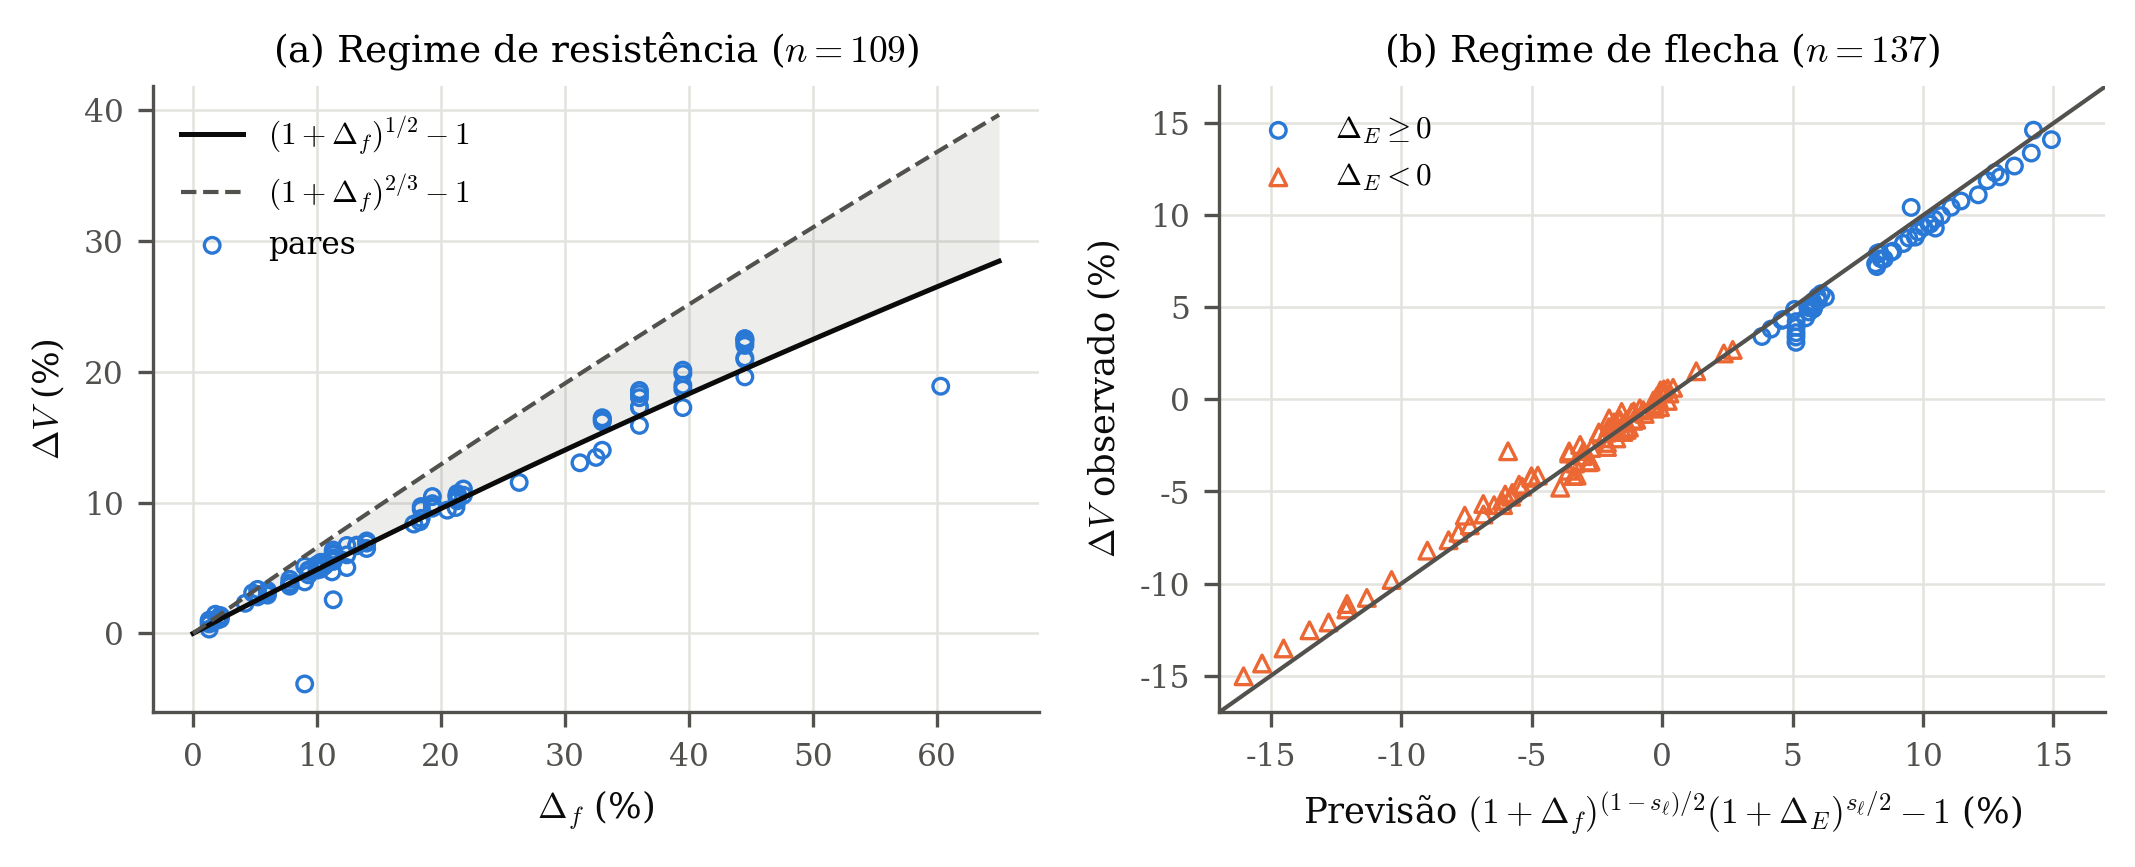
\includegraphics[width=\textwidth]{figuras/res_leis_escala.png}
\caption{Diferença de volume entre o projeto pela classe e pela espécie contra as leis de escala sem parâmetros ajustados: (a) regime de resistência, com a faixa da Equação~\eqref{eq:escala_resistencia}; (b) regime de flecha, com a previsão da Equação~\eqref{eq:escala_flecha}.}
\label{fig:res_escala}
\end{figure}

No regime de flecha, com 137 pares, a rigidez passa a ter o maior peso ($b_E=0{,}322\pm0{,}009$), a resistência mantém uma contribuição menor ($b_f=0{,}160\pm0{,}008$) e a densidade tem efeito pequeno ($b_\rho=-0{,}037\pm0{,}014$). A fração de volume nas longarinas desses projetos tem mediana de 0,68, entre 0,57 e 0,75, o que leva, pela Equação~\eqref{eq:escala_flecha}, a expoentes esperados de cerca de 0,34 para a rigidez e 0,16 para a resistência, praticamente os valores ajustados. Aplicada par a par com a fração de volume de cada projeto, a Equação~\eqref{eq:escala_flecha} reproduz a diferença de volume com viés de 0,02\%, erro quadrático médio de 0,73\% e erro máximo de 3,2\% (Figura~\ref{fig:res_escala}b), sem nenhum parâmetro ajustado. Os pares com $\Delta_E<0$ ocupam o quadrante negativo da figura: são exatamente os pares em que o projeto pela classe usa menos madeira e viola o limite de serviço.

O regime misto, com 74 pares em que apenas um dos projetos do par está no regime de flecha, é o de menor aderência ($R^2=0{,}81$), como esperado, porque nele a mudança de propriedades desloca o próprio regime governante entre os dois projetos.

\subsection{Mapa de decisão entre espécie e classe}\label{sec:res_decisao}

A Figura~\ref{fig:res_decisao} combina os dois passos do critério da Seção~\ref{sec:escala} sobre o plano $\Delta_f\times\Delta_E$, vão a vão. Cada par é classificado em uma de três situações: o projeto pela classe viola o limite de serviço com a espécie; o projeto pela classe é admissível, mas o projeto pela espécie economiza mais de 5\% de madeira; ou a diferença de volume não passa de 5\%.

\begin{figure}[!ht]
\centering
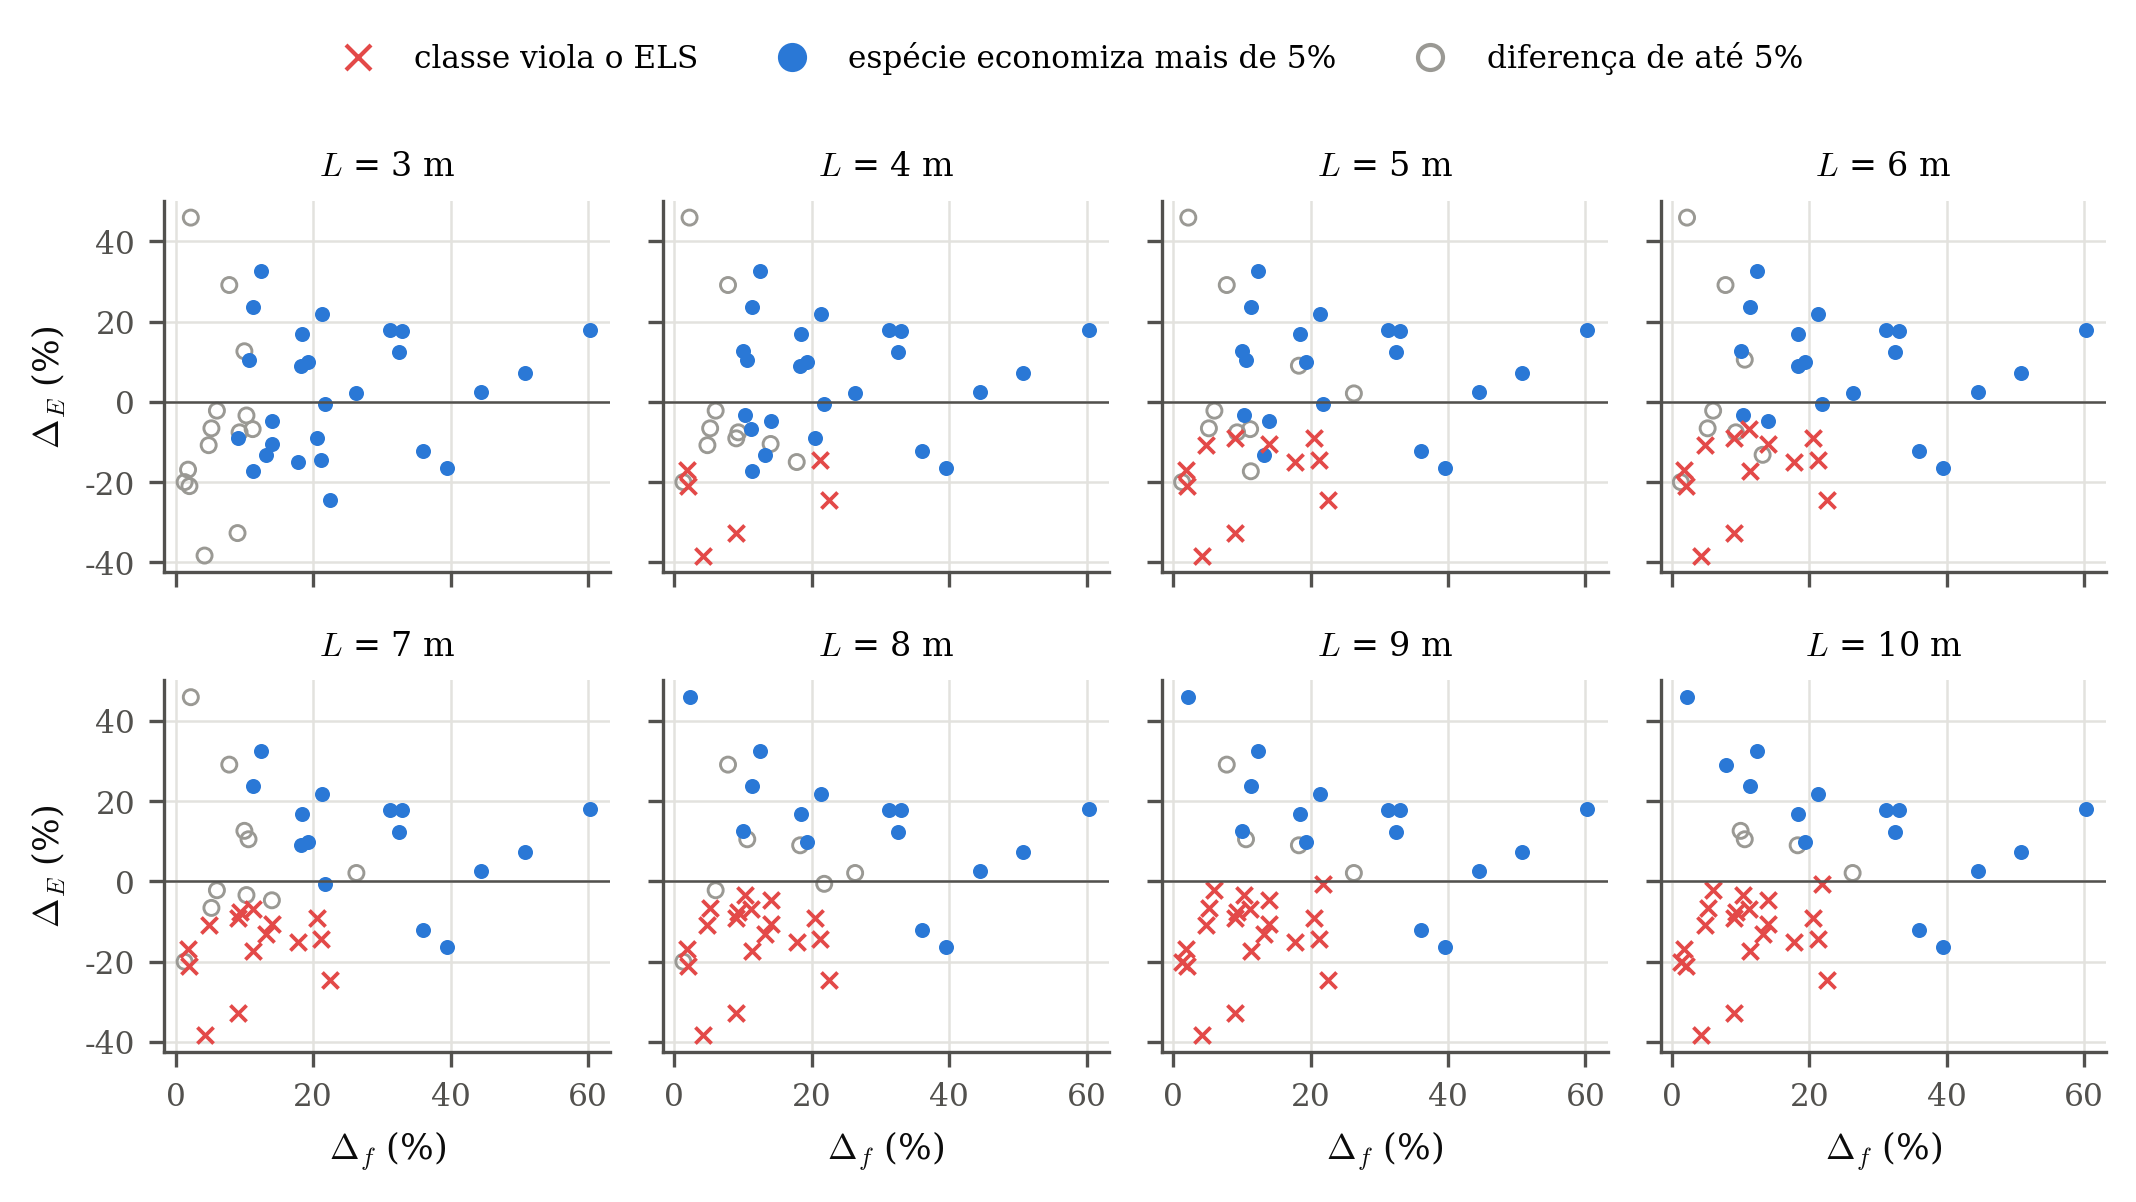
\includegraphics[width=\textwidth]{figuras/res_mapa_decisao.png}
\caption{Mapa de decisão entre o projeto pela espécie e pela classe, por vão, no plano da margem de resistência $\Delta_f$ e do desvio de rigidez $\Delta_E$ de cada espécie em relação à sua classe.}
\label{fig:res_decisao}
\end{figure}

O mapa tem uma estrutura que muda com o vão, mas que se descreve com as duas grandezas do plano. No vão de 3~m, nenhum par viola o limite, e a separação entre economia e indiferença é praticamente vertical, fixada pela margem de resistência: com $\tau=5\%$ e $b_f=1/2$, a Equação~\eqref{eq:escala_resistencia} leva a $\Delta_f^\ast=(1+\tau)^2-1\approx10\%$. Nesse vão, 26 das 40 espécies economizam mais de 5\%, praticamente as mesmas 27 cuja margem de resistência supera $\Delta_f^\ast$. A partir de 4~m, surge abaixo do eixo $\Delta_E=0$ uma região de violação que cresce com o vão e, em 9 e 10~m, ocupa quase todo o semiplano inferior. Acima do eixo, em 10~m, o projeto pela espécie economiza mais de 5\% em 15 espécies, com margem de resistência mediana de 31\% e rigidez mediana 18\% acima da classe. Entre os 215 pares admissíveis, a previsão das Equações~\eqref{eq:escala_resistencia} e~\eqref{eq:escala_flecha} acerta de que lado do limiar de 5\% está cada par em 180 casos. Dos 35 erros, 18 estão no regime misto, e 25 ocorrem em pares cuja diferença de volume fica a menos de dois pontos percentuais do próprio limiar.

Do ponto de vista do projetista, a leitura é direta. Nos vãos em que o projeto pela classe tem folga de flecha maior que o déficit de rigidez possível da espécie, a classe é segura, e a caracterização da espécie é uma decisão econômica, que compensa aproximadamente quando a margem de resistência supera 10\% para uma economia de 5\%. Nos vãos e classes em que o projeto pela classe opera com a flecha no limite, qualquer espécie com módulo inferior ao da classe produz uma ponte que excede o limite de serviço, e a caracterização da rigidez deixa de ser uma questão de economia para ser uma condição de adequação do projeto. Nesta base, isso ocorre para 21 das 40 espécies em algum vão da faixa estudada.

\subsection{Limitações}\label{sec:limitacoes}

A base experimental corresponde a 40 espécies e aos ensaios reportados por \textcite{DiasLahr2004}; não representa automaticamente todos os lotes comerciais dessas espécies. Os dados são agregados por espécie, sem resultados individuais nem covariâncias entre propriedades, de modo que o estudo compara valores representativos e não trata a variabilidade dentro de cada espécie. A resistência característica ao cisalhamento das espécies foi estimada a partir da média publicada, mas o cisalhamento ficou longe do limite em toda a campanha, com utilização máxima de 0,49 na reavaliação.

O modelo estrutural é analítico e restrito a uma superestrutura de vão único simplesmente apoiada, sem ligações, encontros e fundações. Na formulação adotada, a flecha devida à carga variável considera as cargas de roda, mas não a parcela de multidão que atua no momento fletor para $L>6$~m, o que subestima a flecha dos vãos maiores e tende a adiar a entrada no regime de flecha. Como os dois projetos de cada par usam o mesmo modelo, essa simplificação afeta pouco a diferença de volume, mas pode tornar conservadora a contagem de violações. O limiar de 0,99 que define o regime de flecha e o limiar econômico $\tau=5\%$ são escolhas de apresentação; o critério de segurança da Equação~\eqref{eq:criterio} não depende de nenhum deles. As recomendações permanecem restritas à tipologia, às ações, à faixa de vãos e às hipóteses efetivamente avaliadas.
